% Source: :contentReference[oaicite:0]{index=0}
\documentclass{article}
\usepackage{amsmath}
\usepackage{amssymb}
\usepackage{graphicx}
\usepackage{tikz}
\usepackage{pgfplots}
\pgfplotsset{compat=1.18}
\usepackage{booktabs}
\usepackage{xcolor}

\newenvironment{lesson-meta}{}{}        % lesson code, title, objective, EQ, vocab
\newenvironment{item-analysis}{}{}      % Savvas's Example × DOK table
\newenvironment{model-discuss}{}{}      % Launch opener
\newenvironment{concept-box}{}{}        % in-lesson concept reference
\newenvironment{concept-summary}{}{}    % end-of-lesson summary
\newenvironment{example}[1]{}{}         % #1 = example number
\newenvironment{tryit}[1]{}{}           % #1 = tryit number
\newenvironment{practice}[2]{}{}        % #1 = practice number, #2 = DOK
\newenvironment{te-addendum}[2]{}{}     % #1 = anchor example, #2 = type
\newcommand{\answer}[1]{}               % answer key, inside any env
\newcommand{\placeholder}[2]{}          % #1 = type, #2 = description
\newcommand{\uncertain}[2]{#1}          % #1 = best guess, #2 = alternatives
\newcommand{\te}[1]{}                   % teacher-only inline annotation

\begin{document}

\begin{lesson-meta}
Lesson code: 6-3

Title: Logarithms

I CAN: evaluate and simplify logarithms.

Essential Question: What are logarithms and how are they evaluated?

Lesson vocabulary: common logarithm; logarithm; logarithmic function; natural logarithm; natural logarithmic function.

Topic vocabulary: exponential function; inverse function.
\end{lesson-meta}

\begin{item-analysis}
\begin{tabular}{lll}
\toprule
Example & Items & DOK \\
\midrule
1 & 19--22 & 1 \\
2 & 23--30 & 1 \\
3 & 31--38 & 1 \\
  & 16, 55, 56 & 2 \\
  & 17 & 3 \\
4 & 39--44 & 1 \\
  & 13, 15, 18 & 3 \\
5 & 14, 45--50 & 2 \\
6 & 51--54 & 2 \\
  & 57 & 3 \\
\bottomrule
\end{tabular}
\end{item-analysis}

\begin{model-discuss}
CRITIQUE \& EXPLAIN

Earthquakes make seismic waves through the ground. The equation \(y=10^x\) relates the height, or amplitude, in microns, of a seismic wave, \(y\), and the power, or magnitude, \(x\), of the ground-shaking it can cause.

\begin{tabular}{cc}
\toprule
Magnitude, \(x\) & Amplitude, \(y\) \\
\midrule
2 & 100 \\
3 & 1,000 \\
? & 5,500 \\
4 & 10,000 \\
\bottomrule
\end{tabular}

Taylor and Chen used different methods to find the magnitude of the earthquake with amplitude 5,500.

\begin{tabular}{p{0.45\linewidth}p{0.45\linewidth}}
\toprule
Taylor & Chen \\
\midrule
5,500 is halfway between 1,000 and 10,000. & \(y=10^x\) \\
3.5 is halfway between 3 and 4. & \(10^3=1{,}000\) \\
The magnitude is about 3.5. & \(10^4=10{,}000\) \\
 & \(10^{3.5}\approx3{,}162\) \\
 & \(10^{3.7}\approx5{,}012\) \\
 & \(10^{3.8}\approx6{,}310\) \\
 & \(10^{3.74}\approx5{,}500\) \\
 & The magnitude is about 3.74. \\
\bottomrule
\end{tabular}

A. What is the magnitude of an earthquake with amplitude 100,000? How do you know?

B. Construct Arguments Critique Taylor's and Chen's work. Is each method valid? Could either method be improved?

C. Describe how to express the exact value of the desired magnitude.

\answer{A. An earthquake with amplitude 100,000 has a magnitude of 5 because \(10^5=100{,}000\). B. Taylor's method gives a rough estimate, but it is not valid if you need to find a more precise value. Chen's method gives a much closer approximation, although guess and check is not the most efficient way to solve problems. C. The exact value of the magnitude is the value of \(x\) when \(10^x=5500\).}
\end{model-discuss}

\begin{te-addendum}{ModelDiscuss}{LearnTogether}
Q: What do you notice about the relationship between the magnitude and the amplitude of an earthquake?
\answer{As \(x\) increases by 1, \(y\) increases by a power of 10.}

Q: How are Taylor and Chen's work alike?
\answer{Both students made estimates and both may have initially thought that \(x\) would be halfway between 3 and 4. However, Chen used the equation to check and refine his answer.}

Q: When would each student's method of solving the problem be more appropriate?
\answer{Use Taylor's method when an estimate is acceptable. Use Chen's method when a more precise answer is needed.}

For Early Finishers

Q: Use the method you prefer to find the magnitude of an earthquake with amplitude 400.
\answer{\(10^{2.425}\approx400\), \(10^{2.5}\approx316\), \(10^{2.6}\approx398\); The magnitude of an earthquake with amplitude 400 is about 2.6.}

Q: How would you solve the equation \(y=10^x\)?
\answer{Substitute 5,500 for \(y\) and solve for \(x\).}

Q: Can you apply the same method to solve this equation? Explain.
\answer{No; \(y=10^x\) cannot be solved by dividing both sides by 10 because \(x\) is an exponent, not a factor.}
\end{te-addendum}

\begin{te-addendum}{ModelDiscuss}{HabitsOfMind}
Reason Taylor reasoned that since 5,500 was halfway between 1,000 and 10,000 that the magnitude had to be halfway between 3 and 4. What is incorrect about Taylor's reasoning?
\answer{Exponential functions increase exponentially, so they do not increase at a constant rate. There is more growth between \(10^{3.5}\) and \(10^4\) than between \(10^3\) and \(10^{3.5}\).}
\end{te-addendum}

\begin{example}{1}
CONCEPTUAL UNDERSTANDING

ESSENTIAL QUESTION What are logarithms and how are they evaluated?

Understand Logarithms

Solve \(2^x=8\).

Division is the inverse of multiplication, so you can divide both sides by 2 to solve the equation.
\[
\frac{2x}{2}=\frac{8}{2}\qquad x=4
\]

The operation in \(2^x=8\) is exponentiation. To solve this equation, you need an inverse operation that answers the question, ``To what exponent would you raise the base 2 to get 8?''

A logarithm is the inverse of exponentiation. To solve the equation \(2^x=8\), you can write \(\log_2 8=x\). Solving this gives \(\log_2 8=3\) because \(2^3=8\).

This is read ``logarithm base 2 of 8'' or ``log base 2 of 8.''

USE STRUCTURE Creating the notation \(\log_2 x\) to represent the exponent to which you raise 2 to get \(x\) is similar to creating the radical notation \(\sqrt{x}\) to represent one number you can square to get \(x\).

The logarithm base \(b\) of \(x\) is defined as follows.
\[
\log_b x=y \text{ if and only if } b^y=x, \text{ for } b>0,\ b\neq1,\text{ and } x>0.
\]
The logarithmic function \(y=\log_b x\) is the inverse of the exponential function \(y=b^x\).

\answer{\(x=3\)}
\end{example}

\begin{tryit}{1}
Write the logarithmic form of \(y=8^x\).
\answer{\(x=\log_8 y\)}
\end{tryit}

\begin{te-addendum}{1}{PurposefulQuestions}
Q: How is solving \(2x=8\) similar to solving \(2^x=8\)? different?
\answer{Similar: both use inverse operations; different: inverse operation used to solve \(2x=8\) is division and inverse operation used to solve \(2^x=8\) is a logarithm.}

Q: You can calculate the value of \(x\) in \(2^x=8\) without rewriting the function as \(\log_2 8=x\). When might it be necessary to use this notation?
\answer{It will be necessary to use the inverse form of an exponential function to solve more difficult problems.}
\end{te-addendum}

\begin{concept-box}
Exponential and Logarithmic Forms

Exponential form shows that a base raised to an exponent equals the result.
\[
a^b=c
\]
Logarithmic form shows that the log of the result with the given base equals the exponent.
\[
\log_a c=b
\]
When written in logarithmic form, the number that was the result of the exponential equation is often called the argument.
\end{concept-box}

\begin{example}{2}
Convert Between Exponential and Logarithmic Forms

A. What is the logarithmic form of \(3^4=81\)?

The base is 3, the exponent is 4, and the result is 81.

So, in logarithmic form,
\[
3^4=81 \rightarrow \log_3 81=4.
\]
The logarithmic form of \(3^4=81\) is \(\log_3 81=4\).

B. What is the exponential form of \(\log_{10} 1{,}000=3\)?

The base is 10, the exponent is 3, and the result (or argument) is 1,000.

So, in exponential form,
\[
\log_{10} 1{,}000=3 \rightarrow 10^3=1{,}000.
\]
The exponential form of \(\log_{10} 1{,}000=3\) is \(10^3=1{,}000\).

STUDY TIP A fact family for 2, 3, and 5 are the four addition and subtraction equations that relate the three numbers. Think of exponential and logarithmic forms as a fact family for the three numbers given.

\answer{A. \(\log_3 81=4\). B. \(10^3=1{,}000\).}
\end{example}

\begin{tryit}{2}
a. What is the logarithmic form of \(7^3=343\)?

b. What is the exponential form of \(\log_4 16=2\)?

\answer{a. \(\log_7 343=3\) b. \(4^2=16\)}
\end{tryit}

\begin{te-addendum}{2}{PurposefulQuestions}
Q: Why might you find it necessary to convert from one representation of the relationship in an exponential or logarithmic equation to the other?
\answer{Both representations include the same information. One form may be preferred when a problem asks you to solve for a variable.}

Q: What are the exponential and logarithmic equations that show how 2, 5, and 25 are related?
\answer{Use 5 as the base, 2 as the exponent and 25 as the result; \(5^2=25\); \(\log_5 25=2\).}
\end{te-addendum}

\begin{te-addendum}{2}{CommonError}
Try It 3 Some students confuse the placement of the various numbers when converting to another form of the equation.

Instead of writing \(2^5=32\) as \(\log_2 32=5\), students may write the logarithmic form as \(\log_2 5=32\).

Show different parts of the expression using colors or a diagram.
\end{te-addendum}

\begin{te-addendum}{2}{HabitsOfMind}
Communicate Precisely Write a sentence to describe what the equation \(\log_a b=c\) means.
\answer{\(b\) is equal to \(a\) raised to the \(c\)th power.}
\end{te-addendum}

\begin{te-addendum}{2}{RtIExtend}
USE WITH EXAMPLE 2 Give advanced students an extra challenge by asking them to rewrite exponential and logarithmic equations that contain variables.

Q: Rewrite \(y=x^5\) in logarithmic form.
\answer{\(\log_x y=5\)}

Q: Rewrite \(\log_3(n+2)=n-5\).
\answer{\(3^{n-5}=n+2\)}

Q: What value of \(n\) makes the equation \(\log_3(n+2)=n-5\) true?
\answer{7}
\end{te-addendum}

\begin{te-addendum}{2}{PurposefulQuestions}
Additional Example 2A What is the logarithmic form of \(\left(\frac{1}{3}\right)^{-3}=27\)?

The base is \(\frac{1}{3}\). The exponent is \(-3\). The result is 27.
\[
\log_{\frac{1}{3}}27=-3
\]

Q: Does the fact that the base is a fraction change how you write the equation in logarithmic form?
\answer{No; The base of the logarithmic form will be a fraction instead of a whole number, but the structure remains the same.}
\end{te-addendum}

\begin{example}{3}
Evaluate Logarithms

What is the value of each logarithmic expression?

\begin{tabular}{p{0.47\linewidth}p{0.47\linewidth}}
A. \(\log_5 125\) & B. \(\log_{\frac14} 16\) \\
THINK: \(5^?=125\) & THINK: \(\left(\frac14\right)^?=16\) \\
Since \(5^3=125\), \(\log_5 125=3\). & Since \(\left(\frac14\right)^{-2}=16\), \(\log_{\frac14}16=-2\). \\
\midrule
C. \(\log_3 0\) & D. \(\log_2 2^8\) \\
THINK: \(3^?=0\) & THINK: \(2^?=2^8\) \\
There is no such power, so \(\log_3 0\) is undefined. & Since \(2^8=2^8\), \(\log_2 2^8=8\). \\
\end{tabular}

GENERALIZE The output of any exponential function of the form \(y=b^x\), with \(b>0\), is always a positive number. Therefore, the input of a logarithmic function must also be a positive number. Why?

\answer{A. 3 B. \(-2\) C. undefined D. 8}
\end{example}

\begin{tryit}{3}
What is the value of each logarithmic expression?

\begin{tabular}{lll}
a. \(\log_3\left(\frac{1}{81}\right)\) & b. \(\log_7(-7)\) & c. \(\log_5 5^9\)
\end{tabular}

\answer{a. \(-4\) b. undefined c. 9}
\end{tryit}

\begin{te-addendum}{3}{PurposefulQuestions}
Q: Must all parts of a logarithmic expression be positive?
\answer{No; The base must be positive by definition. The input value must be positive because any positive number raised to an exponent yields a positive number. But the properties of exponents state that \(a^{-b}=\frac{1}{a^b}\), so the value of the expression as a whole can be negative.}
\end{te-addendum}

\begin{te-addendum}{3}{ElicitEvidence}
Q: How is Part a in the Try It different from Part B of the example?
\answer{In the Try It, the argument is a fraction, but in the example, the base is a fraction.}
\end{te-addendum}

\begin{concept-box}
Common Logarithms and Natural Logarithms

The base 10 logarithm is called the common logarithm and is written as \(\log x\) with the base of 10 implied.

The base \(e\) logarithm is called the natural logarithm and is written as \(\ln x\).
\end{concept-box}

\begin{example}{4}
Evaluate Common and Natural Logarithms

What is the value of each logarithmic expression to the nearest ten-thousandth?

A. \(\log 900\)
\[
\log 900\approx2.9542
\]
\[
10^{2.9542}\approx900
\]

B. \(\ln e\)
\[
\ln e=1
\]
\[
e^1=e
\]

C. \(\ln(-1.87)\)
\[
\ln(-1.87)\rightarrow \text{ERROR}
\]
There is no exponent to which \(e\) can be raised in order to get a negative number, so \(\ln(-1.87)\) is undefined.
\[
e^?=-1.87
\]

STUDY TIP Scientific calculators have keys for the common logarithm (LOG) and the natural logarithm (LN).

\placeholder{illustration}{Calculator display showing log(900) = 2.954242509, ln(e) = 1, and ln(-1.87) = Error.}

\answer{A. 2.9542 B. 1 C. undefined}
\end{example}

\begin{tryit}{4}
What is the value of each logarithmic expression to the nearest ten-thousandth?

\begin{tabular}{lll}
a. \(\log 321\) & b. \(\ln 1{,}215\) & c. \(\log 0.17\)
\end{tabular}

\answer{a. 2.5065 b. 7.1025 c. \(-0.7696\)}
\end{tryit}

\begin{te-addendum}{4}{PurposefulQuestions}
Q: Why can the exponential form of the expression be used to check your answers?
\answer{The exponential form of the expression is the inverse of the logarithmic form. The exponential form can be used to check logarithmic form in the same way that multiplication can be used to check division.}
\end{te-addendum}

\begin{te-addendum}{3--4}{HabitsOfMind}
Reason For \(\log x\) or \(\ln x\) to be defined, what must be true of \(x\)?
\answer{\(x>0\)}
\end{te-addendum}

\begin{te-addendum}{3}{RtISupport}
USE WITH EXAMPLE 3 Some students may have difficulty understanding how thinking of a logarithmic expression in terms of an exponential equation can help them evaluate logarithms.

Q: What does evaluate mean?
\answer{find the value of}

Q: Must an expression include a variable in order to be evaluated?
\answer{No, numerical expressions can be evaluated.}

Q: If you were asked to evaluate three times four, would it be okay to write ``\(3\times4=?\)''?
\answer{yes}

Q: Can you combine the same logic, along with your knowledge of how to convert between exponential and logarithmic forms, to evaluate \(\log_4 64\)? Explain.
\answer{yes; \(\log_4 64=?\) means \(4^?=64\); \(4^3=64\), so \(\log_4 64=3\).}
\end{te-addendum}

\begin{example}{5}
Solve Equations With Logarithms

What is the solution to each equation? Round to the nearest thousandth.

A. \(25=10^{x-1}\)
\begin{align*}
25&=10^{x-1} \\
\log 25&=x-1 && \text{Convert to logarithmic form.}\\
1+\log 25&=x \\
2.398&\approx x
\end{align*}

B. \(\ln(2x+3)=4\)
\begin{align*}
\ln(2x+3)&=4 \\
2x+3&=e^4 && \text{Convert to exponential form.}\\
2x+3&\approx54.598 \\
2x&\approx51.598 \\
x&\approx25.799
\end{align*}

COMMON ERROR Remember that 10 is not a coefficient, but a base. You cannot divide both sides by 10 and then add 1 to solve for \(x\).

\answer{A. \(x\approx2.398\) B. \(x\approx25.799\)}
\end{example}

\begin{tryit}{5}
Solve each equation. Round to the nearest thousandth.

\begin{tabular}{ll}
a. \(\log(3x-2)=2\) & b. \(e^{x+2}=8\)
\end{tabular}

\answer{a. 34 b. 0.079}
\end{tryit}

\begin{te-addendum}{5}{PurposefulQuestions}
Q: How is solving exponential and logarithmic equations similar to solving linear equations? How is it different?
\answer{Solving any type of equation requires the use of inverse operations. To solve linear equations, you use the inverse operations of addition/subtraction and multiplication/division. To solve exponential equations, you use logarithms, and vice versa.}
\end{te-addendum}

\begin{te-addendum}{5}{CommonError}
Remember that 10 is not a coefficient, but a base. You cannot divide both sides by 10 and then add 1 to solve for \(x\).
\end{te-addendum}

\begin{te-addendum}{5}{PurposefulQuestions}
Additional Example 5 Solve \(4^{6x}=18\). Round to the nearest thousandth.
\begin{align*}
6x&=\log_4 18\\
6x&\approx2.085\\
x&\approx0.347
\end{align*}

Q: How would the solution be different if the 3 were a coefficient of \(e\) rather than a coefficient of \(x\)?
\answer{The first step would be to divide both sides of the equation by 3 before converting to logarithmic form.}
\end{te-addendum}

\begin{example}{6}
APPLICATION

Use Logarithms to Solve Problems

The seismic energy, \(x\), in joules can be estimated based on the magnitude, \(m\), of an earthquake by the formula \(x=10^{1.5m+12}\). What is the magnitude of an earthquake with a seismic energy of \(4.2\times10^{20}\) joules?

\begin{tabular}{p{0.18\linewidth}p{0.72\linewidth}}
Formulate & Substitute \(4.2\times10^{20}\) for \(x\) in the formula. \\
& \(4.2\times10^{20}=10^{1.5m+12}\) \\
Compute & Solve the equation for \(m\). \\
& \(4.2\times10^{20}=10^{1.5m+12}\) \\
& Rewrite in logarithmic form. \\
& \(\log(4.2\times10^{20})=1.5m+12\) \\
& \(20.6\approx1.5m+12\) \\
& \(5.75\approx m\) \\
Interpret & The magnitude of the earthquake is about 5.75. \\
& Verify the answer: \(10^{1.5(5.75)+12}\approx4.2\times10^{20}\). \\
\end{tabular}

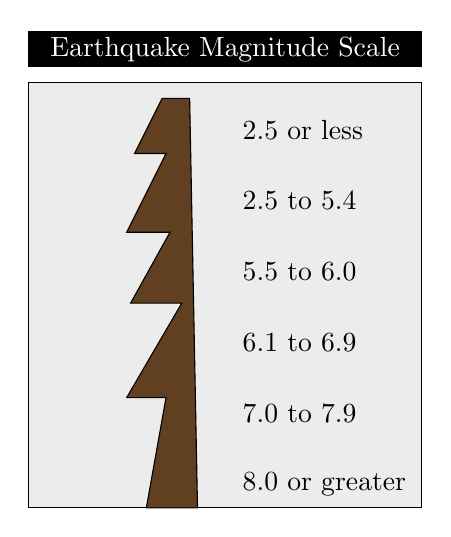
\begin{tikzpicture}
\draw[fill=black] (0,0) rectangle (5,0.45);
\node[text=white] at (2.5,0.225) {Earthquake Magnitude Scale};
\draw[fill=gray!15] (0,-0.2) rectangle (5,-5.6);
\foreach \y/\label in {-0.8/{2.5 or less},-1.7/{2.5 to 5.4},-2.6/{5.5 to 6.0},-3.5/{6.1 to 6.9},-4.4/{7.0 to 7.9},-5.3/{8.0 or greater}}
  \node[anchor=west] at (2.6,\y) {\label};
\draw[fill=brown!50!black] (1.7,-0.4) -- (1.35,-1.1) -- (1.75,-1.1) -- (1.25,-2.1) -- (1.8,-2.1) -- (1.3,-3.0) -- (1.95,-3.0) -- (1.25,-4.2) -- (1.75,-4.2) -- (1.5,-5.6) -- (2.15,-5.6) -- (2.05,-0.4) -- cycle;
\end{tikzpicture}

\answer{The magnitude of the earthquake is about 5.75.}
\end{example}

\begin{tryit}{6}
What is the magnitude of an earthquake with a seismic energy of \(1.8\times10^{23}\) joules?
\answer{magnitude 7.5}
\end{tryit}

\begin{te-addendum}{6}{PurposefulQuestions}
Q: How does converting the form of the equation help to find the magnitude of the earthquake?
\answer{The equation can be converted from exponential form to a linear equation containing a logarithm. The logarithm can be evaluated and the linear equation can be solved in two more steps to reveal the magnitude.}
\end{te-addendum}

\begin{te-addendum}{6}{ElicitEvidence}
Q: Do you think the magnitude of the earthquake in the Try It will be greater than or less than the magnitude of the earthquake in the example?
\answer{It will be greater because \(1.8\times10^{23}>4.2\times10^{20}\).}
\end{te-addendum}

\begin{te-addendum}{5--6}{HabitsOfMind}
Reason How do logarithms help you solve an equation in which the variable is an exponent?
\answer{It allows you to rewrite the expression in terms of the variable.}
\end{te-addendum}

\begin{te-addendum}{6}{ELLAddendum}
READING BEGINNING Explain to students that the word joules is a homophone. Homophones are words that have the same pronunciation but different meanings and spellings. Write the words joules and jewels, along with their respective definitions, on the board. Provide sentences in which students fill in the blank either with joules or jewels.

Q: There are 20 \underline{\hspace{1cm}} in the king's crown.
\answer{jewels}

Q: A heavy-duty surge protector will protect all of your electronic devices from surges up to 5,500 \underline{\hspace{1cm}}.
\answer{joules}

LISTENING DEVELOPING Place some small objects on a desk and use a magnifying glass to look at them.

Q: What is a magnifying glass used for?
\answer{to make small objects look larger}

Q: What do the words magnify, magnificent, and magnitude have in common?
\answer{the prefix magni-}

Q: What do you think the prefix magni- means, and how does it help you to understand the meaning of the word magnitude?
\answer{large; The magnitude of an earthquake is a measure of how large it is.}

WRITING EXPANDING Ask students to write the definitions of seismic energy, joules, and magnitude. Then have them draw a diagram to show the connections between the words.

Q: Explain how seismic energy is related to joules and to magnitude.
\answer{Seismic energy is measured in joules. There is a strong positive correlation between seismic energy and the magnitude of an earthquake.}
\end{te-addendum}

\begin{concept-summary}
Logarithms

\begin{tabular}{p{0.12\linewidth}p{0.36\linewidth}p{0.36\linewidth}}
\toprule
 & Exponential Form & Logarithmic Form \\
\midrule
ALGEBRA & \(b^x=y\) & \(\log_b y=x\) \\
WORDS & The base raised to the exponent is equal to a result. & The logarithm with a base \(b\) of the result (or argument) is equal to the exponent. \\
NUMBERS & \(3^4=81\) & \(\log_3 81=4\) \\
\bottomrule
\end{tabular}

Do You UNDERSTAND?

1. ESSENTIAL QUESTION What are logarithms and how are they evaluated?
\answer{Logarithms are exponents. Logarithms can be evaluated by rewriting them in exponential form.}

2. Error Analysis Amir said the expression \(\log_5(-25)\) simplifies to \(-2\). Explain Amir's possible error.
\answer{Amir possibly brought the negative sign outside the expression, which is not an equivalent step.}

3. Vocabulary Explain the difference between the common logarithm and the natural logarithm.
\answer{Common logarithms use the base 10. Natural logarithms use the base \(e\).}

4. Make Sense and Persevere How can logarithms help to solve an equation such as \(10^t=656\)?
\answer{You can convert the equation to logarithmic form, \(t=\log 656\), which also solves the equation.}

Do You KNOW HOW?

Write each equation in logarithmic form.

5. \(2^{-6}=\frac{1}{64}\)
\answer{\(\log_2\left(\frac{1}{64}\right)=-6\)}

6. \(e^4\approx54.6\)
\answer{\(\ln 54.6\approx4\)}

Write each equation in exponential form.

7. \(\log 200\approx2.301\)
\answer{\(10^{2.301}\approx200\)}

8. \(\ln 25\approx3.22\)
\answer{\(e^{3.22}\approx25\)}

Evaluate the expression.

9. \(\log_4 64\)
\answer{3}

10. \(\log\frac{1}{100}\)
\answer{\(-2\)}

11. \(\ln e^5\)
\answer{5}

12. Solve for \(x\). \(4e^x=7\).
\answer{\(\ln\left(\frac{7}{4}\right)\), or 0.5596}
\end{concept-summary}

\begin{te-addendum}{ConceptSummary}{PurposefulQuestions}
Q: Explain the relationship between logarithms and exponents.
\answer{Logarithms and exponents are inverse operations.}

Q: When is it useful to convert between exponential and logarithmic forms?
\answer{It is useful to rewrite an exponential equation in logarithmic form when the exponent contains a variable. The logarithm can be evaluated and the resulting linear equation can easily be solved. Similarly, it is useful to rewrite a logarithmic equation in exponential form when the result (or argument) contains a variable. The exponent, with a base of 10 or \(e\), can be evaluated and the resulting linear equation can easily be solved.}
\end{te-addendum}

\begin{te-addendum}{ConceptSummary}{CommonError}
Exercise 11 Some students may think that \(e\) is a variable and not a constant. Explain that \(e\) is an irrational number called Euler's number. Compare \(e\) to \(\pi\) to help students understand that \(e\) represents a specific number that is approximately 2.718.
\end{te-addendum}

\begin{practice}{13}{3}
Make Sense and Persevere If the LN button on your calculator were broken, how could you still use your calculator to find the value of the expression \(\ln 65\)?
\answer{Graph \(y=e^x\) and use the graph to find an approximate value of \(x\) for which \(y\) is equal to 65.}
\end{practice}

\begin{practice}{14}{2}
Error Analysis Describe and correct the error a student made in solving an exponential equation.
\[
\begin{aligned}
16e^t&=98\\
e^t&=6.125\\
6.125t&=\ln e\\
t&=\frac{\ln e}{6.125}
\end{aligned}
\]
\answer{The student did not convert to logarithmic form correctly. The solution should be \(t=\ln 6.125\).}
\end{practice}

\begin{practice}{15}{3}
Higher Order Thinking Use the graph of \(y=3^x\) to estimate the value of \(\log_3 50\). Explain your reasoning.

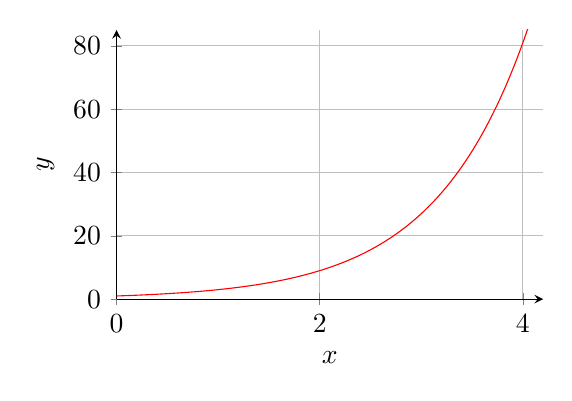
\begin{tikzpicture}
\begin{axis}[
axis lines=left,
xmin=0,xmax=4.2,
ymin=0,ymax=85,
width=7cm,height=5cm,
xlabel={$x$},ylabel={$y$},
xtick={0,2,4},ytick={0,20,40,60,80},
grid=both,
]
\addplot[red, domain=0:4.05, samples=120] {3^x};
\end{axis}
\end{tikzpicture}

\answer{3.5; \(\log_3 50\) is an expression equivalent to \(3^x=50\), so you need to find the value of \(x\) for which \(y=50\).}
\end{practice}

\begin{practice}{16}{2}
Generalize For what values of \(x\) is the expression \(\log_4 x<0\) true?
\answer{\(\{x\mid0<x<1\}\)}
\end{practice}

\begin{practice}{17}{3}
Use Structure A student says that \(\log_3\left(\frac{1}{27}\right)\) simplifies to \(-3\). Is the student correct? Explain.
\answer{yes; \(3^{-3}=\frac{1}{27}\)}
\end{practice}

\begin{practice}{18}{3}
Use Structure Explain why the expression \(\ln 1{,}000\) is not equal to 3.
\answer{Because the base is \(e\) and \(e^3\) is not equal to 1,000.}
\end{practice}

\begin{practice}{19}{1}
Construct Arguments Explain why \(\log_b b^x=x\). Explain why \(e^{\ln x}=x\).
\answer{\(y=\log_b x\) and \(y=b^x\) are inverses. Part of the definition of inverses is that \(f(g(x))=x=g(f(x))\). It follows that \(\log_b b^x=x\). Since \(y=e^x\) and \(y=\ln x\) are inverses, then the same reasoning applies for \(e^{\ln x}=x\).}
\end{practice}

\begin{practice}{20}{1}
Write the logarithmic form of the exponential equation. SEE EXAMPLE 1

\(y=4^x\)
\answer{\(\log_4 y=x\)}
\end{practice}

\begin{practice}{21}{1}
Write the logarithmic form of the exponential equation. SEE EXAMPLE 1

\(y=10^x\)
\answer{\(\log y=x\)}
\end{practice}

\begin{practice}{22}{1}
Write the logarithmic form of the exponential equation. SEE EXAMPLE 1

\(y=7^x\)
\answer{\(\log_7 y=x\)}
\end{practice}

\begin{practice}{23}{1}
Write the logarithmic form of the exponential equation. SEE EXAMPLE 1

\(y=a^x\)
\answer{\(\log_a y=x\)}
\end{practice}

\begin{practice}{24}{1}
Write each equation in logarithmic form. SEE EXAMPLE 2

\(3^8=6{,}561\)
\answer{\(\log_3 6561=8\)}
\end{practice}

\begin{practice}{25}{1}
Write each equation in logarithmic form. SEE EXAMPLE 2

\(e^{-3}\approx0.0498\)
\answer{\(\ln 0.0498=-3\)}
\end{practice}

\begin{practice}{26}{1}
Write each equation in logarithmic form. SEE EXAMPLE 2

\(5^0=1\)
\answer{\(\log_5 1=0\)}
\end{practice}

\begin{practice}{27}{1}
Write each equation in logarithmic form. SEE EXAMPLE 2

\(7^3=343\)
\answer{\(\log_7 343=3\)}
\end{practice}

\begin{practice}{28}{1}
Write each equation in exponential form. SEE EXAMPLE 2

\(\log\frac{1}{100}=-2\)
\answer{\(10^{-2}=\frac{1}{100}\)}
\end{practice}

\begin{practice}{29}{1}
Write each equation in exponential form. SEE EXAMPLE 2

\(\log_8 64=2\)
\answer{\(8^2=64\)}
\end{practice}

\begin{practice}{30}{1}
Write each equation in exponential form. SEE EXAMPLE 2

\(\ln 148.41\approx5\)
\answer{\(e^5\approx148.41\)}
\end{practice}

\begin{practice}{31}{1}
Write each equation in exponential form. SEE EXAMPLE 2

\(\log_2\frac{1}{32}=-5\)
\answer{\(2^{-5}=\frac{1}{32}\)}
\end{practice}

\begin{practice}{32}{1}
Evaluate each logarithmic expression. SEE EXAMPLE 3

\(\log_5\frac{1}{125}\)
\answer{\(-3\)}
\end{practice}

\begin{practice}{33}{1}
Evaluate each logarithmic expression. SEE EXAMPLE 3

\(\log_6(-216)\)
\answer{undefined}
\end{practice}

\begin{practice}{34}{1}
Evaluate each logarithmic expression. SEE EXAMPLE 3

\(\log_3 3^4\)
\answer{4}
\end{practice}

\begin{practice}{35}{1}
Evaluate each logarithmic expression. SEE EXAMPLE 3

\(\log_2 32\)
\answer{5}
\end{practice}

\begin{practice}{36}{1}
Evaluate each logarithmic expression. SEE EXAMPLE 3

\(\log_9 729\)
\answer{3}
\end{practice}

\begin{practice}{37}{1}
Evaluate each logarithmic expression. SEE EXAMPLE 3

\(\log_8\frac{1}{64}\)
\answer{\(-2\)}
\end{practice}

\begin{practice}{38}{1}
Evaluate each logarithmic expression. SEE EXAMPLE 3

\(\log_7 0\)
\answer{undefined}
\end{practice}

\begin{practice}{39}{1}
Evaluate each logarithmic expression. SEE EXAMPLE 3

\(\log_7 7^a\)
\answer{\(a\)}
\end{practice}

\begin{practice}{40}{1}
Use a calculator to evaluate each expression. Round to the nearest ten-thousandth. SEE EXAMPLE 4

\(\log 78.5\)
\answer{1.8949}
\end{practice}

\begin{practice}{41}{1}
Use a calculator to evaluate each expression. Round to the nearest ten-thousandth. SEE EXAMPLE 4

\(\log 0.24\)
\answer{\(-0.6198\)}
\end{practice}

\begin{practice}{42}{1}
Use a calculator to evaluate each expression. Round to the nearest ten-thousandth. SEE EXAMPLE 4

\(\ln(-37)\)
\answer{undefined}
\end{practice}

\begin{practice}{43}{1}
Use a calculator to evaluate each expression. Round to the nearest ten-thousandth. SEE EXAMPLE 4

\(\ln 41.5\)
\answer{3.7257}
\end{practice}

\begin{practice}{44}{1}
Use a calculator to evaluate each expression. Round to the nearest ten-thousandth. SEE EXAMPLE 4

\(\log 12\)
\answer{1.0792}
\end{practice}

\begin{practice}{45}{2}
Use a calculator to evaluate each expression. Round to the nearest ten-thousandth. SEE EXAMPLE 4

\(\ln 3\)
\answer{1.0986}
\end{practice}

\begin{practice}{46}{2}
Solve each equation. Round answers to the nearest ten-thousandth. SEE EXAMPLES 5 AND 6

\(\log(7x+6)=3\)
\answer{142}
\end{practice}

\begin{practice}{47}{2}
Solve each equation. Round answers to the nearest ten-thousandth. SEE EXAMPLES 5 AND 6

\(2.75e^t=38.6\)
\answer{2.6417}
\end{practice}

\begin{practice}{48}{2}
Solve each equation. Round answers to the nearest ten-thousandth. SEE EXAMPLES 5 AND 6

\(\ln(3x-1)=2\)
\answer{2.7964}
\end{practice}

\begin{practice}{49}{2}
Solve each equation. Round answers to the nearest ten-thousandth. SEE EXAMPLES 5 AND 6

\(10^{t+1}=50\)
\answer{0.6990}
\end{practice}

\begin{practice}{50}{2}
Solve each equation. Round answers to the nearest ten-thousandth. SEE EXAMPLES 5 AND 6

\(1.5e^t=27\)
\answer{2.8904}
\end{practice}

\begin{practice}{51}{2}
Solve each equation. Round answers to the nearest ten-thousandth. SEE EXAMPLES 5 AND 6

\(\log(x-3)=-1\)
\answer{3.1}
\end{practice}

\begin{practice}{52}{2}
How long does it take for \$250 to grow to \$600 at 4\% annual percentage rate compounded continuously? Round to the nearest year.
\answer{22 years}
\end{practice}

\begin{practice}{53}{2}
Model with Mathematics Michael invests \$1,000 in an account that earns a 4.75\% annual percentage rate compounded continuously. Peter invests \$1,200 in an account that earns a 4.25\% annual percentage rate compounded continuously. Which person's account will grow to \$1,800 first?
\answer{Peter's account}
\end{practice}

\begin{practice}{54}{2}
Reason The Richter magnitude of an earthquake is \(R=0.67\log(0.37E)+1.46\), where \(E\) is the energy (in kilowatt-hours) released by the earthquake.

\placeholder{photo}{Cracked wall photo with Richter scale overlay numbered 1 through 10 and labels ``Not felt'' at 1 and ``Extreme'' near 9--10; callout text: ``At a richter magnitude of 4 and above, the walls in your house may start to crack.''}

a. What is the magnitude of an earthquake that releases 11,800,000,000 kilowatt-hours of energy? Round to the nearest tenth.

b. How many kilowatt-hours of energy would earthquake have to release in order to be an 8.2 on the Richter scale? Round to the nearest whole number.

c. What number of kilowatt-hours of energy would an earthquake have to release in order for walls to crack? Round to the nearest whole number.

\answer{a. magnitude 7.9 b. 31,009,857,353 kWh c. 16,705 kWh}
\end{practice}

\begin{practice}{55}{2}
Reason The function \(c(t)=108e^{-0.08t}+75\) calculates the temperature, in degrees Fahrenheit, of a cup of coffee that was handed out a drive-thru window \(t\) minutes ago.

a. What is the temperature of the coffee in the instant that it is handed out the window?

b. After how many minutes is the coffee in the cup 98 degrees Fahrenheit? Round to the nearest whole minute.

\answer{a. \(183^{\circ}\mathrm{F}\) b. 19 minutes}
\end{practice}

\begin{practice}{56}{2}
Sheba invests \$500 in an account that earns 2.5\% annual percentage rate compounded continuously. How long will it take for her account to grow to \$700?
\answer{about \(13\frac{1}{2}\) years}
\end{practice}

\begin{practice}{57}{3}
SAT/ACT In the equation \(\log_3 a=b\), if \(b\) is a whole number, which of the following CANNOT be a value for \(a\)?

\begin{tabular}{ccccc}
A. 1 & B. 3 & C. 6 & D. 9 & E. 81
\end{tabular}

\answer{6}
\end{practice}

\begin{practice}{58}{\uncertain{not listed}{Item Analysis omits Performance Task 58}}
Performance Task Money is deposited into two separate accounts. The money in one account is compounded continuously. The money in the other account is not compounded continuously. Neither account has any money withdrawn in the first 6 years.

\begin{tabular}{ccc}
\toprule
Year & Account 1 Balance (\$) & Account 2 Balance (\$) \\
\midrule
0 & 400 & 500 \\
1 & 433.31 & 575 \\
2 & 469.40 & 650 \\
3 & 508.50 & 725 \\
4 & 550.85 & 800 \\
5 & 596.72 & 875 \\
\bottomrule
\end{tabular}

Part A Write a function to calculate the amount of money in each account given \(t\), the number of years since the account was opened. Describe the growth in each account.

Part B Will the amount of money in Account 1 ever exceed the amount of money in Account 2? Explain. If so, when will that occur?

\answer{a. Account 1: \(A=400e^{0.08t}\). Account 2: \(A=500+75t\). b. yes; Account 2 is increasing at a constant rate while Account 1 is increasing at an increasing rate, so after a certain point the amount of money in Account 1 will exceed the amount of money in Account 2; in about 20 years.}
\end{practice}

\end{document}